\section{AI辅助3D建模}


AI在3D建模中的应用,如同为创意插上了科技的翅膀,为设计领域带来了前所未有的变革。它不仅极大地提升了建模效率,还为设计师们提供了更广阔的创作空间。借助AI,即使是复杂的3D模型也能在短时间内生成,大大减少了传统手工建模所需的繁琐步骤和时间成本。AI的智能算法能够根据简单的描述或图像快速生成高质量的模型框架,并自动优化结构和纹理,确保模型的精确度和美观度。这种技术不仅降低了3D建模的门槛,让非专业人士也能轻松上手,还能在游戏开发、影视制作、建筑设计、产品设计等多个领域快速响应需求变化,节省大量时间和成本。未来,随着AI技术的不断发展,其在3D建模中的应用将更加广泛,有望为创意产业带来更多的创新和变革,为设计师们提供更强大的工具,推动整个行业的发展。


\textbf{案例:基础3D建模}
本案例通过AI工具快速实现Blender软件中的3D场景原型搭建,为不用3D建模的读者提供快速上手的可能。下面给出与AI工具的交互的过程,可在Blender软件中生成红色正方体,如\reffig{fig:3d-red-cube}所示。

\prompt{写Blender Python脚本:创建一个简单立方体,包含基础灯光和摄像机}


\begin{gptbox} 
\small{ 
\begin{lstlisting}[language=Python] 
import bpy

# 清空场景
bpy.ops.object.select_all(action='SELECT')
bpy.ops.object.delete(use_global=False)

# 创建立方体
bpy.ops.mesh.primitive_cube_add(
    size=2,                # 立方体边长
    location=(0, 0, 0),    # 中心位置
    rotation=(0, 0, 0)     # 初始旋转
)
cube = bpy.context.object
cube.name = "Simple_Cube"  # 命名对象

# 创建基础材质
material = bpy.data.materials.new(name="Cube_Material")
material.diffuse_color = (0.8, 0.1, 0.1, 1)  # RGBA红色
cube.data.materials.append(material)

# 设置摄像机
bpy.ops.object.camera_add(
    location=(5, -5, 3),   # 摄像机位置
    rotation=(1.047, 0, 0.785)  # 60度俯角,45度偏角
)
bpy.context.scene.camera = bpy.context.object

# 添加灯光
bpy.ops.object.light_add(
    type='POINT',
    location=(3, -3, 5),
    radius=1.0
)
bpy.context.object.data.energy = 500  # 灯光强度

# 设置渲染基础参数
bpy.context.scene.render.resolution_x = 1280
bpy.context.scene.render.resolution_y = 720

print("基础立方体场景创建完成!")

\end{lstlisting}
} 
\end{gptbox}

\fig[h]{
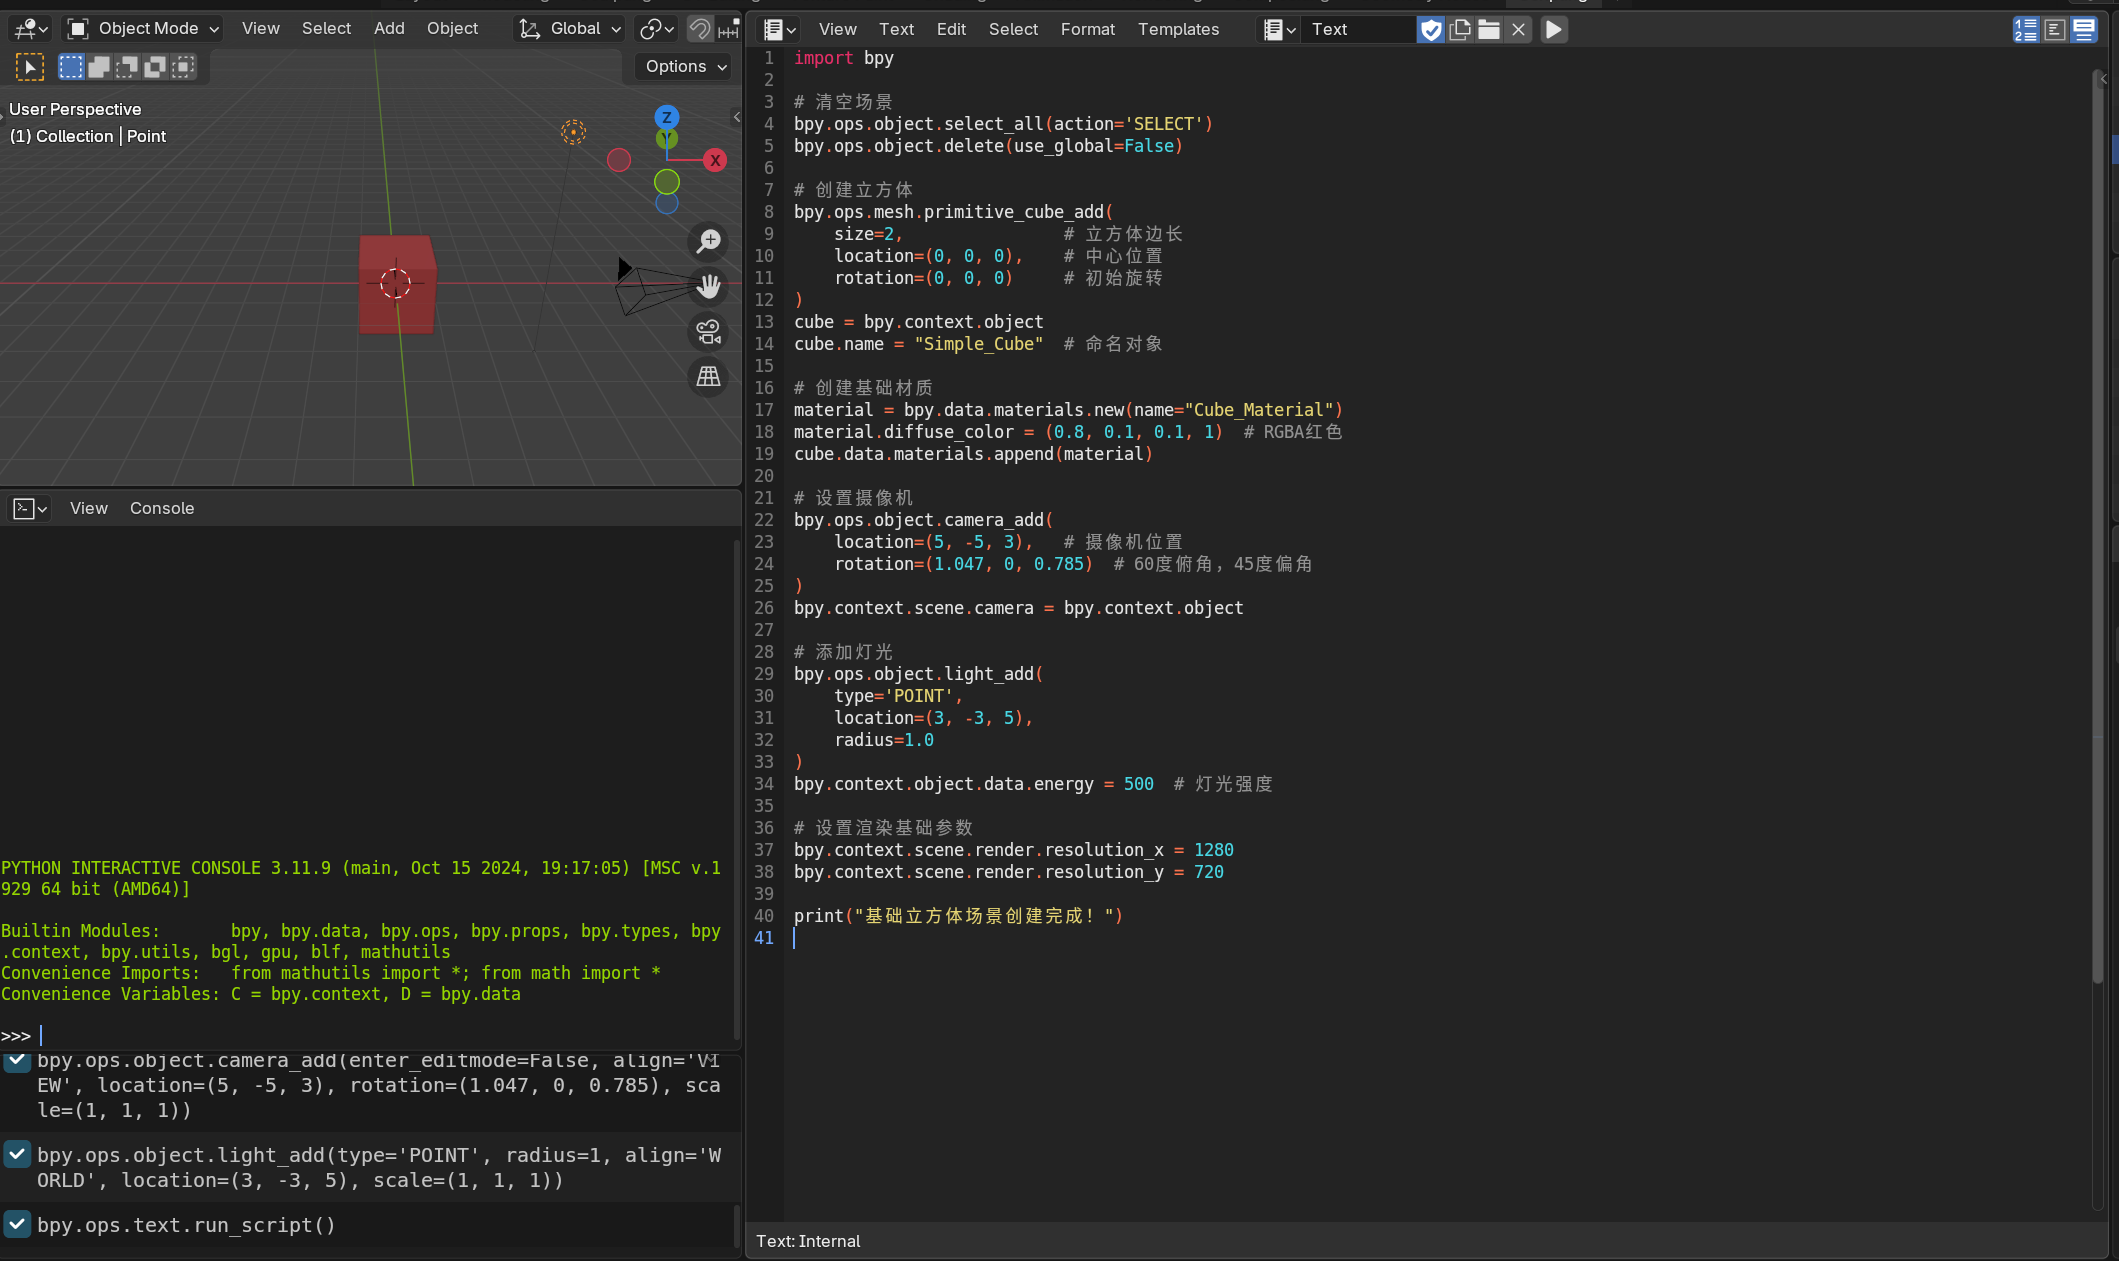
\includegraphics[width=0.7\textwidth]{assets/figures/红色立方体效果图.jpg} %插入图片,[]中设置图片大小,{}中是图片文件名
  \caption{红色立方体效果图} %最终文档中希望显示的图片标题
  \label{fig:3d-red-cube} %用于文内引用的标签
}

接着对现有模型进一步拓展延伸,个性化修改参数。修改后的立方体如\reffig{fig:3d-blue-cube-changed}所示。

\prompt{如何修改立方体尺寸和颜色?}

\begin{gptbox} 
\footnotesize{\# 修改立方体大小为3,修改颜色并添加光照强度和灯光颜色:}
\small{
\begin{lstlisting}[language=Python]
import bpy

# 清空场景
bpy.ops.object.select_all(action='SELECT')
bpy.ops.object.delete(use_global=False)

# 创建立方体
bpy.ops.mesh.primitive_cube_add(
    size=3,                # 立方体边长
    location=(0, 0, 0),    # 中心位置
    rotation=(0, 0, 0)     # 初始旋转
)
cube = bpy.context.object
cube.name = "Simple_Cube"  # 命名对象

# 创建基础材质
material = bpy.data.materials.new(name="Cube_Material")
material.diffuse_color = (0.2, 0.6, 0.9, 1)  # 蓝色
cube.data.materials.append(material)

# 设置摄像机
bpy.ops.object.camera_add(
    location=(5, -5, 3),   # 摄像机位置
    rotation=(1.047, 0, 0.785)  # 60度俯角,45度偏角
)
bpy.context.scene.camera = bpy.context.object

# 添加灯光
bpy.ops.object.light_add(
    type='POINT',
    location=(3, -3, 5),
    radius=1.0
)
bpy.context.object.data.energy = 1000  # 灯光强度
bpy.context.object.data.color = (1, 0.9, 0.8)  # 暖色调灯光

# 设置渲染基础参数
bpy.context.scene.render.resolution_x = 1280
bpy.context.scene.render.resolution_y = 720

print("蓝色立方体修改完成!")

\end{lstlisting}
} 
\end{gptbox} 

\fig[h]{
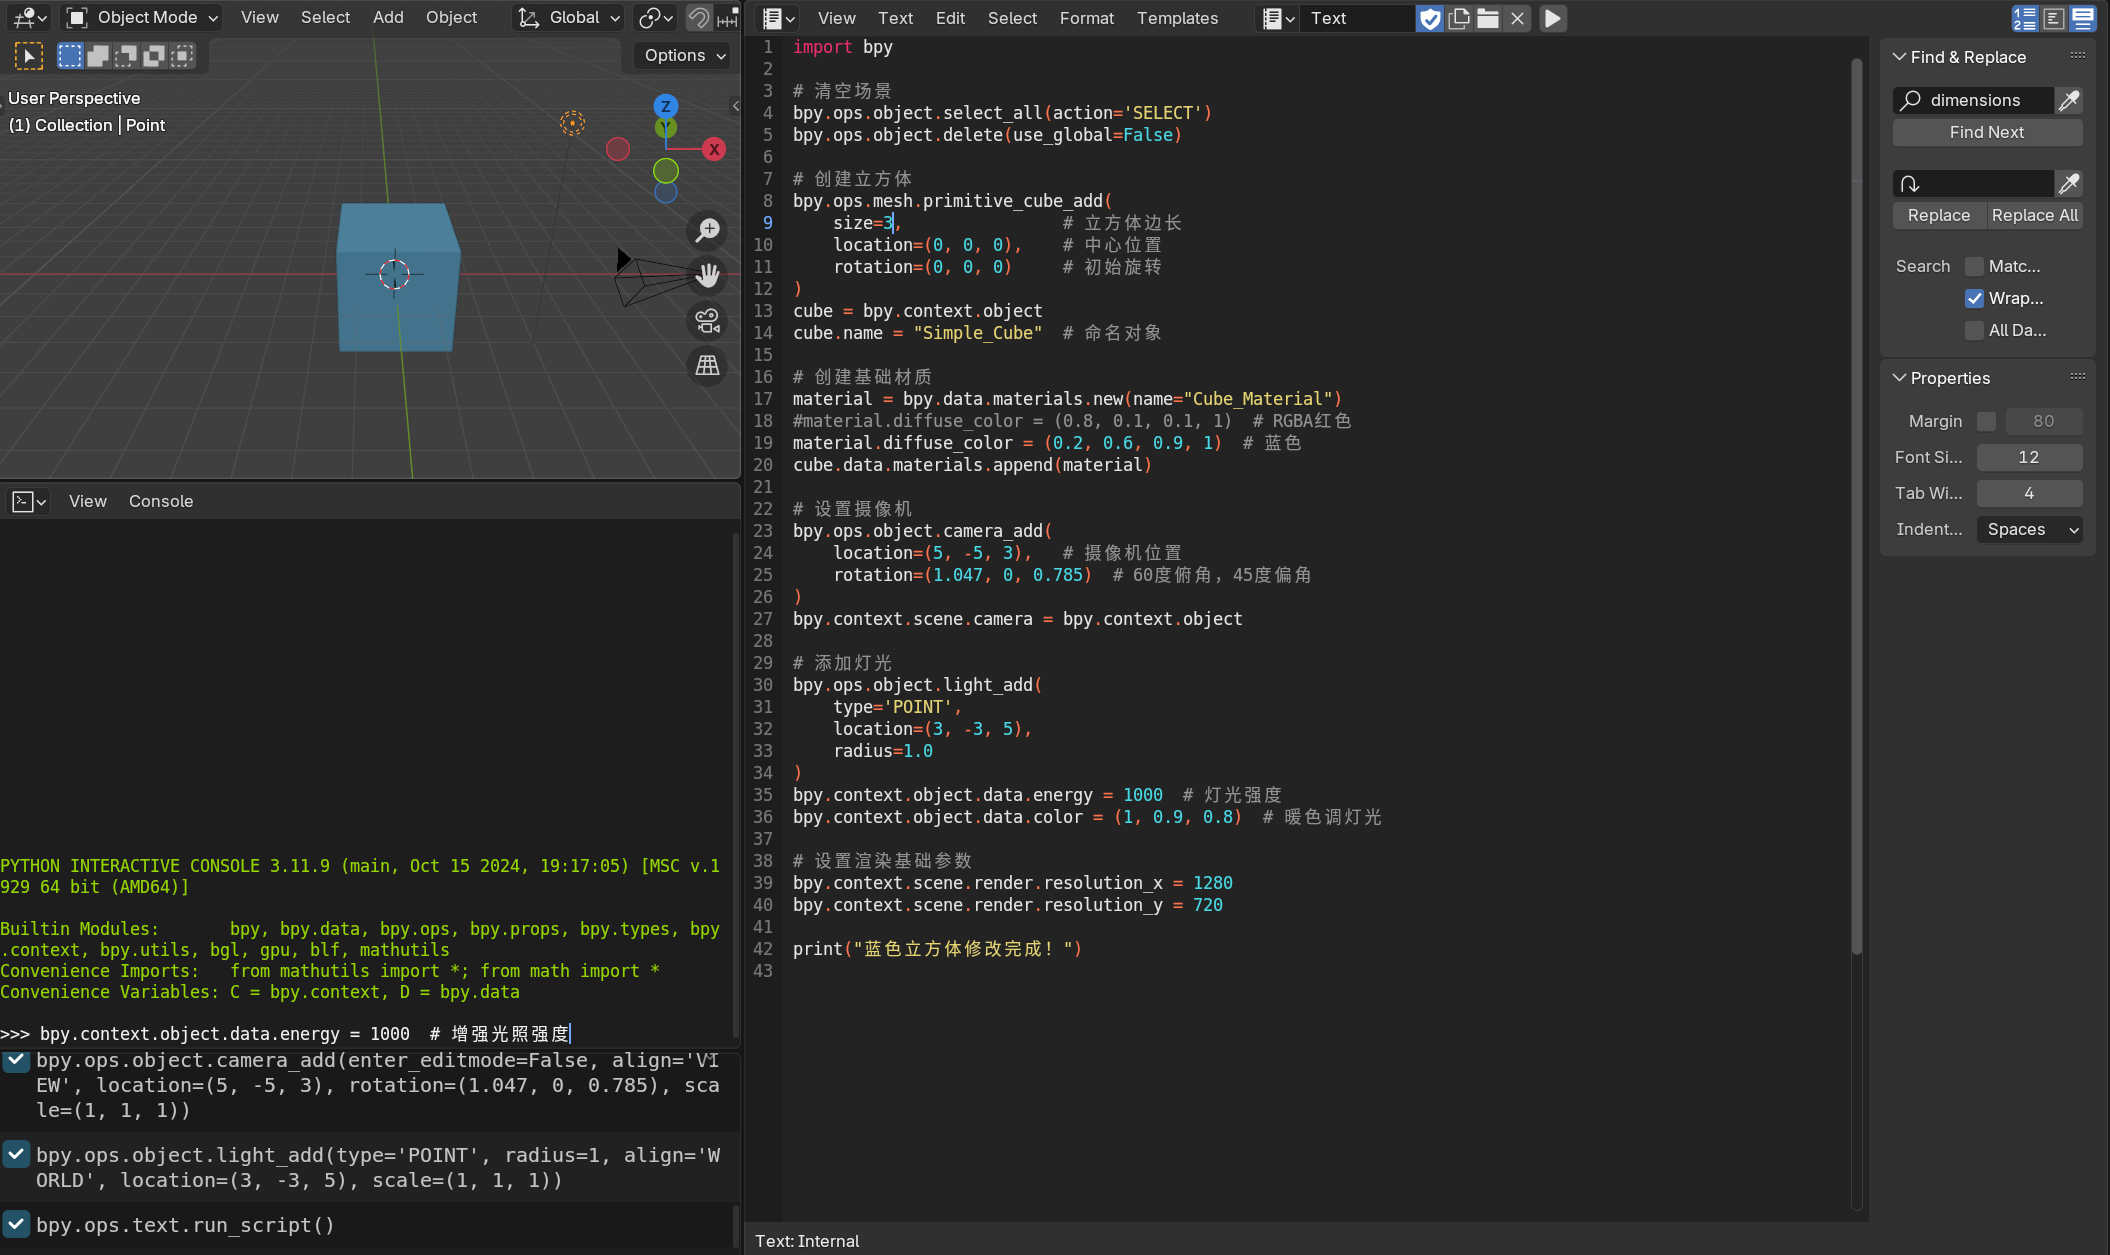
\includegraphics[width=0.7\textwidth]{assets/figures/修改后效果图.jpg} %插入图片,[]中设置图片大小,{}中是图片文件名
  \caption{修改后效果图} %最终文档中希望显示的图片标题
  \label{fig:3d-blue-cube-changed} %用于文内引用的标签
}

\subsection{动手试试看}
AI提示词示例 
改变物体形状:
\prompt{将立方体改为球体}\\
调整场景光照:
\prompt{添加三点照明系统} \\
制作简单动画:
\prompt{创建旋转动画效果} \\